\chapter{Access-Control Views on Blockchain}
\label{ch:view}


\section{Introduction}
\label{ch:view:intro}

There has been a rapid increase in the popularity of blockchains during the last decade. Blockchain was initially introduced as a tamper-proof decentralized ledger for prevention of {\texttt double spending\/} in cryptocurrencies like Bitcoin~\cite{nakamoto2019bitcoin}. However, in recent years many new blockchain applications were developed, in a variety of areas, including healthcare~\cite{dagher2018ancile}, identity management~\cite{dunphy2018first}, financial data management~\cite{guo2016blockchain,cocco2017banking,peters2016understanding,tapscott2017blockchain}, decentralized traffic control~\cite{dasu2018geofences}, tracking IoT devices~\cite{banafa2017iot}, management of personal data~\cite{zyskind2015decentralizing}, supply chain management~\cite{dujak2019blockchain,tse2017blockchain}, etc. Blockchain has become an important tool for managing shared data in applications with no single agreed-upon trusted entity that could store and manage all the data, or in cases where data records should result from a consensus between organizations that do not fully trust each other~\cite{gupta2021fault}.  

Blockchain was initially designed as a transparent ledger, e.g., in cryptocurrencies all the users see all the transactions. Transparency is needed for preventing double spending---a case where a user pays with the same coins in two different transactions. %, by using money that has already been spent. 
However, nowadays blockchain has many uses, not just managing cryptocurrencies. In many applications, the information stored on the blockchain is sensitive and should be concealed from some of the users, including some or all of the peers who manage the blockchain. An example of that is a blockchain application for storing health records~\cite{halamka2017potential}. Such records contain sensitive private information and should not be revealed to unauthorized users. Access to the information should be granted to authorized users, but the set of authorized users could change over time, e.g., new healthcare workers may need access to health records that were stored before they were hired. 

In database management systems, an access control module manages access permissions and prevents unauthorized users from accessing restricted data~\cite{gertz2007handbook}. A similar
system is needed for protecting sensitive information on a blockchain. 
%But there is no similar mechanism for blockchains. 
The following example illustrates the need for access-control views in a blockchain-supported supply chain management system. 
\begin{example}
\label{ch:view:example:supply_chain}
Figure~\ref{diagram:view:supply_chain:} presents a data supply chain with 2 manufacturers, 3 warehouses, 2 delivery services and several shops. The manufacturers, shops and warehouses store information about items they produced or handled. Every delivery transaction is visible to all the entities who handled the item. 
%each shop should have provenance information about the items that were delivered to it, and each warehouse tracks delivery information for items that were stored in it. 
(For instance, to support a recall of products.)
%For items like food or medical supply, improper storage conditions may necessitate executing a recall based on detailed delivery information. 
When there is no single entity that can be trusted to manage all the data, the information could be kept on a blockchain. However, without any access control, all the information is visible to every user. Such a solution does not provide business confidentiality.
%, e.g., requiring that Manufacturer~1 would not see information on items of Manufacturer~2 and vice versa. 
Similarly, each warehouse, shop and delivery service should only be able to see the information pertaining to items they processed, delivered or received. 
\end{example}

Access-control views are used in database management systems for specifying access-control permissions. For example, consider in the supply chain of Example~\ref{ch:view:example:supply_chain}, a view $V_{M1}$ of all the delivery records of items produced by Manufacturer~1 and a view $V_{M2}$ of records related to items produced by Manufacturer~2. Granting Manufacturer~1 access only to $V_{M1}$ and granting Manufacturer~2 access only to $V_{M2}$ would satisfy the business confidentiality requirements. However, there are no such access-control views in blockchains. Furthermore, implementing access-control views on blockchain requires coping with transparency, immutability and  lack of central control, as explained next.

Access to a view is granted or revoked by users who are authorized to do so. In a centralized access-control system, a central system is responsible for enforcing the access-control policy. Guaranteeing that the access-control policy is enforced correctly in a decentralized environment is more challenging. In many applications, the peers who manage the blockchain cannot be fully trusted. Decisions regarding data are based on a consensus mechanism under the assumption that the majority of the peers are honest (trustworthy). But even a single dishonest peer can leak sensitive information. So, it is undesirable to allow all the peers to access sensitive information when not all of them can be trusted.

Another challenge when managing access control on blockchain is to revoke access permissions. The blockchain is immutable, so past records cannot be changed. Designing access control in which access can be revoked should cope with that.
%
Immutability of the blockchain also makes updates of views a challenging task. If views are stored on the ledger, it is impossible to update the view records when the underlying data change. Thus, views on a blockchain should be designed for an append-only ledger. 

In this work, we study access-control views for blockchain. Our main contributions are as follows.
\begin{itemize}
    \item Introducing access-control views for blockchain, where sensitive information can be hidden by either encryption or hashing, based on the user preferences.
    \item Showing how to implement the access-control views and role-based access control (RBAC) in a decentralized environment.
    \item Analyzing the methods and showing that they support verifiable completeness and soundness, that is, a user can verify that each view contains exactly the set of transactions it should consist of according to the view definition.
    \item Presenting a modular system architecture for managing views, querying them and verifying their integrity.
    \item We implemented a workload generator for supply chain applications, for benchmarking the proposed method. 
    \item Extensive experiments over a supply chain workload demonstrate the effectiveness of our approach.
\end{itemize}

Our methods were implemented on Hyperledger Fabric v2.2 but they are generic and can be implemented on other blockchain systems. We assume that user identities are pre-defined and authenticated, so our methods can be directly applied to permissioned blockchains. With any Sybil-resistant consensus algorithm, such as Proof of Work, we can extend our approach to permissionless blockchains. 

\begin{figure}
    \centering
    %\fbox{
    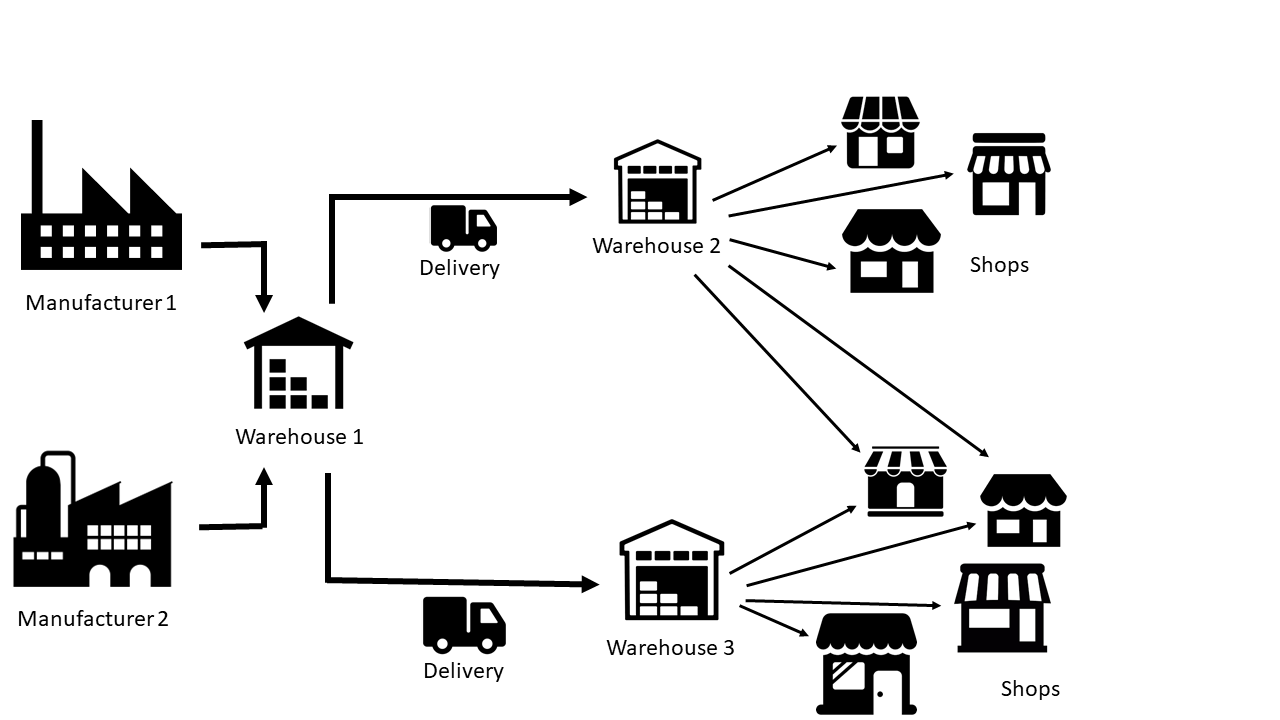
\includegraphics[trim=0 0 150 60, clip,width=0.94\textwidth]{diagram/view/supply_chain.png}
    %}
    \caption{An Illustration of a Supply Chain. }
    \subcaption*{It consists of two manufacturers, three warehouses and several shops. }
    \label{diagram:view:supply_chain:}
\end{figure}

This chapter is organized as follows.
In Chapter~\ref{ch:view:framework} we present our framework and formally define the research problem. Our view methods are presented in Chapter~\ref{ch:view:ac_views}. 
% RBAC is explored in Chapter~\ref{ch:view:rbac}.
In Chapter~\ref{ch:view:impl} we explain how we implemented the proposed methods, and in Chapter~\ref{ch:view:experiments} we present an experimental evaluation of the methods. 


\section{Framework}
\label{ch:view:framework}

\medskip
\noindent
\textbf{Blockchain.}
Blockchain is a ledger managed by peers in a decentralized fashion.
We denote by $P$ the set of peers that manage the blockchain. To simplify the discussion we assume that $P$ does not change over time.
By {\em users\/} we refer to people or applications that access the blockchain. The set of users $U$ consists of peers, which create blocks, and additional users, which may access the blockchain to read the content of blocks but without creating blocks. 
We assume that each user $u\in U$ has a pair of public and private keys, denoted $\pubk{u}$ and $\privk{u}$, in correspondence. This pair of keys can be based on RSA~\cite{rivest1978method} or any other public-key cryptosystem. 



\medskip
\noindent
\textbf{Sensitive information.} %As mentioned above, a 
A blockchain may include sensitive information such as health records, personal documents, financial data and location data. Each transaction $t_{ij}$ has two parts, a non-secret part denoted $t_{ij}[N]$ and a secret part, denoted $t_{ij}[S]$. The non-secret part is visible to all the users and can be used in the consensus protocol, to determine which transactions to include in the blockchain. The access to the secret part should be limited and granted to users according to the access permissions. 
\begin{example}
Suppose that in the supply chain of Example~\ref{ch:view:example:supply_chain} every transfer of items is recorded on the blockchain, e.g., transfers from a manufacturer to a warehouse or from a warehouse to a shop. Each transaction includes shipment data. Details like shipment number, date and the involved entities are included in the non-secret part. The type of items, amount of delivered items and price are confidential and included in the secret part.
\end{example}

All the transactions on the blockchain are visible to all the peers, and thus, the secret part is concealed by either encrypting it or storing on the blockchain just the cryptographic hash of the secret. We elaborate on that in the following chapters.
%, when presenting our view methods. 
The encryption of a secret part can be by a symmetric encryption key like AES~\cite{daemen2001reijndael} or TDEA~\cite{barker2017recommendation}, or using a public key cryptosystem like RSA~\cite{rivest1978method}. As a secure cryptographic hash, SHA-256 can be used~\cite{gueron2011sha}.  We assume that each transaction has a unique identifier, and we denote by $\tid{ij}$ the identifier of transaction $t_{ij}$. Accordingly, a transaction is a 3-tuple $(\tid{ij}, t_{ij}[N], t_{ij}[S])$ of id, non-secret part and secret part.




\medskip
\noindent
\textbf{Granting and revoking access.}
Each transaction is added to the blockchain by some user $u\in U$. We assume that $u$ knows the secret part or the key to decrypt it, for all the transactions $u$ adds to the blockchain. {\texttt Granting access\/} to user $u'$ for transaction $t_{ij}$ is providing the means for $u'$ to see the secret part of $t_{ij}$. {\texttt Revoking access\/} means that the permission to see the secret part is repealed so that a request to access the secret information would be denied.

To grant access to sets of records, it is common to use {\em access-control views}. The view specifies a set of records, and access permissions specify the users who should be allowed to read these records. There are two types of access-control permissions over blockchain, {\texttt revocable\/} and {\texttt irrevocable}. A revocable access permission is similar to standard access control in database management systems---it can be granted and revoked. 
An irrevocable permission cannot be revoked  and it is unique to blockchains. We present and study blockchain views with revocable and irrevocable access permissions.



\medskip
\noindent
\textbf{Verifiable soundness and completeness.}
Given a database $D$ and a query $Q$ over $D$, a view $V$ can be defined as $Q(D)$, that is, the result of applying $Q$ to $D$. If $V$ is a maintained view, the following two properties are required.
{\texttt (1)~Soundness\/}: $V$ is sound if $V\subseteq Q(D)$, and 
{\texttt (2)~completeness\/}: $V$ is complete if $V\supseteq Q(D)$. 

In a decentralized environment, it is not always possible to guarantee soundness and completeness. Thus, we relax the requirement to the ability to verify soundness and completeness of the view at any given time $T$. {\texttt Verifiable soundness\/} and {\texttt verifiable completeness\/} at $T$ are the ability of users with access permissions to $V$ to verify the soundness and completeness of $V$ according to all the transactions that were added to the underlying dataset until time $T$.   


\medskip
\textbf{View definition.}
Typically, views are defined using a query. In a {\em maintained view}, the query answer is stored and updated when there are changes in the underlying data. In a {\em logical view}, the view query is computed when the view is invoked. For access control, we can store on the blockchain a maintained view and grant users access to it, or store on the blockchain only the information regarding who has access to data and provide the data when requested if access is allowed according to the records on the blockchain.

A {\em view definition\/} is a predicate $P_V$ over the non-secret part of transactions. A predicate $P_V$ defines a view $V=\{t_{ij} \mid P_V(t_{ij}[N])\}$ with the set of transactions $t_{ij}$ for which $P_V(t_{ij}[N])$ is true. 

\begin{example}
\label{ch:view:example:view_def}
Consider the supply chain in Example~\ref{ch:view:example:supply_chain}. 
Suppose that each shipment transaction has {\texttt{from}} and {\texttt{to}} attributes, to specify the entities in the shipment. A predicate $P(\texttt{to}) = \textrm{``Warehouse~1''}$ specifies the set of all transactions that are delivered to Warehouse~1. 
\end{example}

The view defined in Example~\ref{ch:view:example:view_def} is local and does not connect transactions to one another, e.g., it cannot relate to the history of item deliveries. To address this, we add recursion to the view definition, in a datalog fashion~\cite{abiteboul1995foundations}. Since datalog programs with recursion are a well known concept, we avoid providing formal definitions here, and only explain the main concepts. 

A datalog {\texttt rule\/} contains a head and body and it is defined in a recursive way. Given a predicate $P(t)$ over transactions, a rule $Q(t) \gets P(t)$ specifies that $Q(t)$ is true for all the transactions that satisfy predicate $P(t)$. In this case, $Q(t)$ is the head of the rule and $P(t)$ is the body of the rule. 

A rule $Q(t)\gets P_1(t), P_2(t), \ldots, P_m(t)$ specifies that $Q$ is satisfied by transactions that satisfy  the predicates $P_1, P_2,\ldots, P_m$. For a set of rules $Q(t)\gets P_1(t)$, $Q(t)\gets P_2(t), \ldots$, $Q(t)\gets P_k(t)$, the transactions satisfying $Q(t)$ are the union $\{ t \mid P_1(t) \vee P_2(t)\vee\ldots P_k(t)\}$ comprising the set of transactions satisfying at least one of the rules. Datalog rules can be recursive. For example, $\texttt{Delivery}(t, \texttt{from}, \texttt{to})$ contains transactions $t$ delivered between the two locations specified by \texttt{to} and \texttt{from}. The following set of rules 
\begin{eqnarray*}
P_1(t, \texttt{from}, \texttt{to}) & \gets & \texttt{Delivery}(t, \texttt{from}, \texttt{``Warehouse 1''}) \\
P_1(t, X, Z) & \gets & \texttt{Delivery}(t, X, Y),  P_1(t_1, Y, Z) \\
P(t) & \gets & P_1(t, X, Y)
\end{eqnarray*}
defines a predicate $P(t)$ of all the transactions that are part of a delivery to ``Warehouse~1''.
%
The predicates can relate to any attribute of the stored transactions or of the blocks that contain them, e.g., transaction time, transaction id, block creation time, block id, etc. 

In many blockchain systems, the data stored on the ledger and the states of smart contracts are maintained in a local database, where a Merkle tree is used for validating the integrity of data and of answers to queries posed to the local database, as explained in Chapter~\ref{ch:view:framework}. By using the local database, a query over the ledger is computed efficiently, e.g., in Hyperledger Fabric, LevelDB or CouchDB are used for storing the state database and answering queries that are posed to the blockchain.


\section{Access-Control Views}
\label{ch:view:ac_views}

In this chapter, we explain how to create views with revocable and irrevocable access permissions. We present four different methods for creating access-control views on blockchain %(see Table~\ref{tab:four:view:types}) 
and we discuss their advantages and disadvantages. In all the methods, we assume that the blockchain peers cannot be fully trusted. Hence, in all the methods, the secret part of transactions is hidden from the peers and only revealed if access to the data is explicitly granted to that peer. First we explain how views are created and used and then we explain how access permissions are granted and revoked.


\subsection{Encryption-based Irrevocable  Permissions}
\label{ch:view:ac_views:enc_irrevocable}

We present now access-control views that are based on encryption and are irrevocable, namely EI. In EI, the secret part of each transaction is stored encrypted and the decryption key is provided only to users who are granted access to the secret information. 

\medskip
\noindent
\textbf{Storing transactions with a secret part.}
Initially, before adding a transaction $t_{ij}$ to the blockchain, the user $u$ who adds the transaction generates a new key $K_{ij}$, and conceals the secret part of  $t_{ij}$ by encrypting it with the key  $K_{ij}$. Each transaction is encrypted with a unique symmetric encryption key. Transaction $t_{ij}$ is stored as a 3-tuple $(\tid{ij}, t_{ij}[N], \enc(t_{ij}[S]), K_{ij})$ of id, non-secret part and encrypted secret part, as illustrated in Figure~\ref{diagram:view:enc_irrevocable}. 

Initially, only user $u$ has the key to see the transaction. To grant access to the secret part of transactions, the keys should be disseminated to authorised users. This is done via access-control views.  

\medskip
\noindent
\textbf{Creating a view.} An access-control view is a list of keys of the transactions it comprises. Suppose that user $u$ wants to grant access to transactions $t_1, \ldots, t_n$. Let $K_1,\ldots,K_n$ be the keys of the transactions $t_1, \ldots, t_n$, in correspondence. To create an access-control view $V$, user $u$ produces a new symmetric key $K_V$. The view $V$ is stored on the blockchain as a list $\enc([\tid{1}, K_1,\ldots, \tid{n}, K_n], K_V)$, that is, the encryption of the keys $K_1,\ldots,K_n$ (and the ids of the corresponding transactions) with the view key $K_V$. The list is stored as a transaction $t_V$. Note that at this point only $u$ knows $K_V$ so no secret information is revealed yet. However, providing the key $K_V$ to a user $u'$ will allow $u'$ to decrypt the content of $t_V$, acquire the keys of  $t_1, \ldots, t_n$, and access the secret parts of these transactions. 

\medskip
\noindent
\textbf{Granting access to a view.} To grant users $u'_1,\ldots, u'_m$ with access to a view $V$, the user $u$ that created $V$ can either send the key to these users via a secured communication channel. Another option is to create and add to the blockchain a transaction that contains the encryption of $K_V$ with the public keys of  $u'_1,\ldots, u'_m$, that is, $\enc(K_V, \pubk{u'_1}), \ldots, \enc(K_V, \pubk{u'_m})$. Each user $u'_i$ will be able to decrypt $\enc(K_V, \pubk{u'_i})$ using the private key $\privk{u'_i}$. Any user who is not among $u'_1,\ldots, u'_m$ will not know the private key for decrypting the content of this dissemination transaction.

The blockchain is an append-only ledger, so all the transactions, including the view and the access to the view, are tamper-resistant and cannot be deleted. Hence, access permissions are irrevocable. 

   
\begin{figure}[t]
    \centering
    %\fbox{
    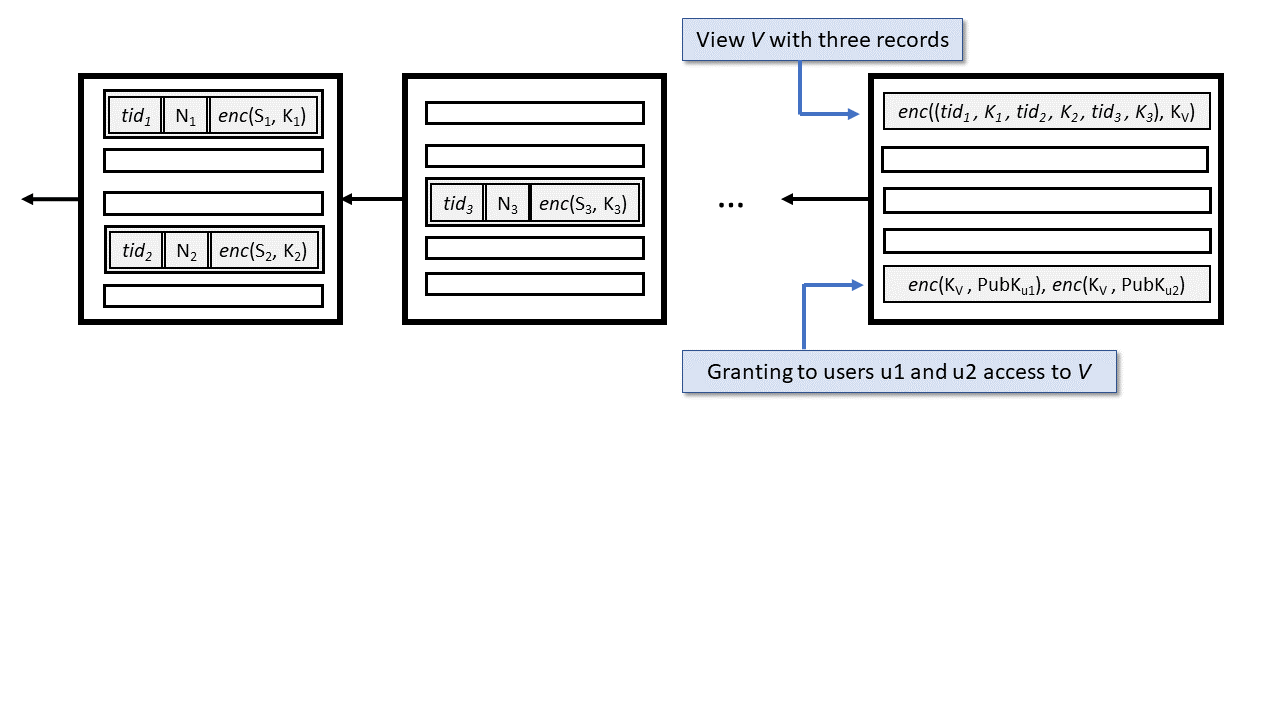
\includegraphics[trim=0 220 0 0, clip,width=0.87\textwidth]{diagram/view/enc_irrevocable.png}
    %}
    \caption{An Encryption-based Irrevocable Access-control View.}
    \subcaption*{View $V$ contains three transactions, $t_1$, $t_2$ and $t_3$. An irrevocable access to the transactions is given to users $u_1$ and $u_2$ by providing to them the keys of $t_1$, $t_2$ and $t_3$ via the view.}
    \label{diagram:view:enc_irrevocable}
\end{figure}




\subsection{Encryption-based Revocable Permissions}
\label{ch:view:ac_views:enc_revocable}

We now describe revocable permissions for an encryption-based
storage of transactions as in Chapter~\ref{ch:view:ac_views:enc_irrevocable}, namely ER.

\medskip
\noindent
\textbf{Creating a view.}
To make the access permission revocable, the secret information should be disseminated in a way that allows denying access when permissions change. The secret information should not be revealed by an immutable blockchain transaction. Instead, the transaction keys should be provided to users with an access permission upon request, as long as the access permission was granted and has not been revoked.

Consider a revocable view $V$ created by user $u$, for transactions $t_1,\ldots, t_n$. Let $u'_1,\ldots, u'_m$ be the users that should have access to the transactions in view $V$.
The user $u$ has access to all the keys of the transactions in $V$, but these keys are not provided to the users $u'_1,\ldots, u'_m$ in an irreversible way. 

To implement revocable access permissions, the view has two parts, $V_{\texttt ids\/}$ and $V_{\texttt access\/}$. The first part is the ids of the transactions the view contains, i.e., $V_{\texttt ids\/} = \{ \tid{1}, \ldots, \tid{n}\}$ is the list of ids of the transactions $t_1,\ldots, t_n$ contained in $V$. 
%
The $V_{\texttt access\/}$ part is used for managing access to the view. User $u$ creates a new key $K_V$ generated for the view. That key is disseminated to the users in an encrypted way as a list $V_{\texttt access\/} = \{\enc(K_V, \pubk{u'_1}), \ldots, \enc(K_V, \pubk{u'_m})\}$. Key $K_V$ is stored in an encrypted way and only a user $u'_i$ who knows the private key $\privk{u'_i}$ can read it. Note, however, that $K_V$ is not a key of any transaction, so knowing it still does not guarantee access to secret information.

The user $u$ who created the view $V$ is considered the {\em view owner\/} and any access to the information on the view is through this user.
%, as explained next.

\medskip
\noindent
\textbf{Granting and revoking access.}
When a user $u'_j$ wants to access transactions $t_{i_1}, \ldots, t_{i_k}$ of view $V$, it requests the keys of transactions $t_{i_1}, \ldots, t_{i_k}$ from $u$. These keys are provided encrypted as $\enc(K_{i_1}, K_V), \ldots, \enc(K_{i_m}, K_V)$. If the user 
$u'_j$ has the key $K_V$, it can decrypt the sent keys and access the transactions. We assume here that $K_V$ is a symmetric encryption key. Note that this does not reveal transaction keys that were not requested.

To grant additional users access to the view, $u$ can share the key $K_V$ with these users, encrypted using their public key.
To revoke access from some users, $u$ needs to replace the key $K_V$ with a new key, say $K'_V$, and disseminate the new key $K'_V$ to the users that still have permission to access $V$. This is done as described above, i.e., by encrypting the new key $K'_V$ with the public keys of the authorized users and including that in the transaction of $V_{\texttt access\/}$ stored on the blockchain. After the change, $u$ should only use $K'_V$ to encrypt requested transaction keys.    Figure~\ref{diagram:view:enc_revocable} illustrates the method. When access is revoked, users may still have access to information they downloaded and stored locally, but they could not access and download additional information.

   
\begin{figure}[t]
    \centering
    %\fbox{
    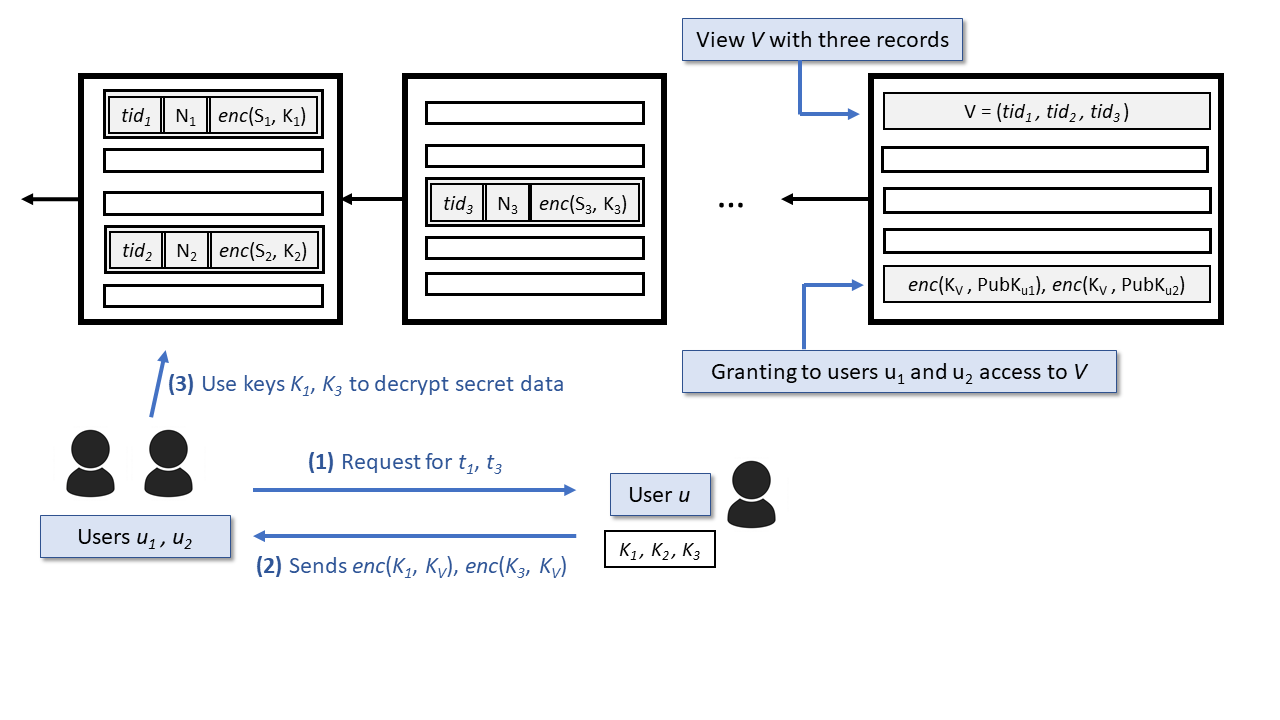
\includegraphics[trim=0 50 0 0, clip,width=0.87\textwidth]{diagram/view/enc_revocable.png}
    %}
    \caption{A Encryption-based Revocable Access-control View. }
    \subcaption*{The users receive a key $K_V$ that allows them to decrypt information of the transactions in the view. The secret values should be requested from the view owner, and these values are provided encrypted using $K_V$. } 
    \label{diagram:view:enc_revocable}
\end{figure}





\subsection{Hash-based Irrevocable Access Permissions}
\label{ch:view:ac_views:hash_irrevocable}

In hash-based views, the secret part of transactions %stored on the blockchain 
is replaced by its hash value. 
%Since for the secret part of transactions only the hash is stored on the ledger, 
To implement irrevocable access control (namely, HI), the secret part of transactions should be revealed only to authorized users. 
%That is, for transactions that are included in the view, their 
The secret part of view transactions is stored in an encrypted view. The decryption key of the view is provided only to users with access permissions to the view. 

\medskip
\noindent
\textbf{Storing transactions with a secret part.}
Initially, before adding a transaction $t_{ij}$ to the blockchain, the user $u$ who adds the transaction conceals the secret part of  $t_{ij}$ by selecting a  random {\texttt salt\/} $s$, computing the hash of $h(t_{ij}[S] \conc s)$, where $t_{ij}[S] \conc s$ is the concatenation of the secret part of $t_{ij}$ with the salt $s$, and storing this hashed value on the blockchain instead of storing $t_{ij}[S]$ itself. The salt prevents seeing that two secret values are the same in two different transactions, to prevent a Dictionary Attack. Each transaction $t_{ij}$ is stored as a 4-tuple $(\tid{ij}, t_{ij}[N], s_{ij}, h(t_{ij}[S] \conc s_{ij}))$ of id, non-secret part, salt and hash of salt and secret part. 

Initially, only user $u$ has the secret values of transactions. To grant access to the secret part of transactions, these values are disseminated to authorised users, via the access-control views.  

\medskip
\noindent
\textbf{Creating a view.}
Suppose that user $u$ wants to grant access to transactions $t_1, \ldots, t_n$.
Before the view is created, only the hash values $h(t_1[S]\conc s_1), \ldots, h(t_n[S]\conc s_n)$ of the secret parts of the transactions are stored on the blockchain. To create a view $V$ and grant access to the secret parts of transactions $t_1, \ldots, t_n$, user $u$ creates a new key $K_V$, and stores on the blockchain the encrypted content
$\enc((\tid{1}, t_{1}[S]), K_V), \ldots, \enc((\tid{n}, t_{n}[S]), K_V)$. 

\medskip
\noindent
\textbf{Granting access to the view.}
The key $K_V$ and salts $s_i$ are 
distributed to all the users with access permissions to view $V$. If user $u'$ receives from $u$ the key $K_V$, then $u'$ can decrypt $t_1[S], \ldots, t_n[S]$ and verify that their hash values concatenated with the salt are equal to the hash values $h(t_1[S]\conc s_1), \ldots, h(t_n[S]\conc s_n)$ stored on the blockchain.
Note that access to the data is irrevocable because if $u'$ has the key $K_V$ then that key reveals the secret part of each transaction in the view. The method is illustrated in Figure~\ref{diagram:view:hash_irrevocable}.

\begin{figure}[t]
    \centering
    %\fbox{
    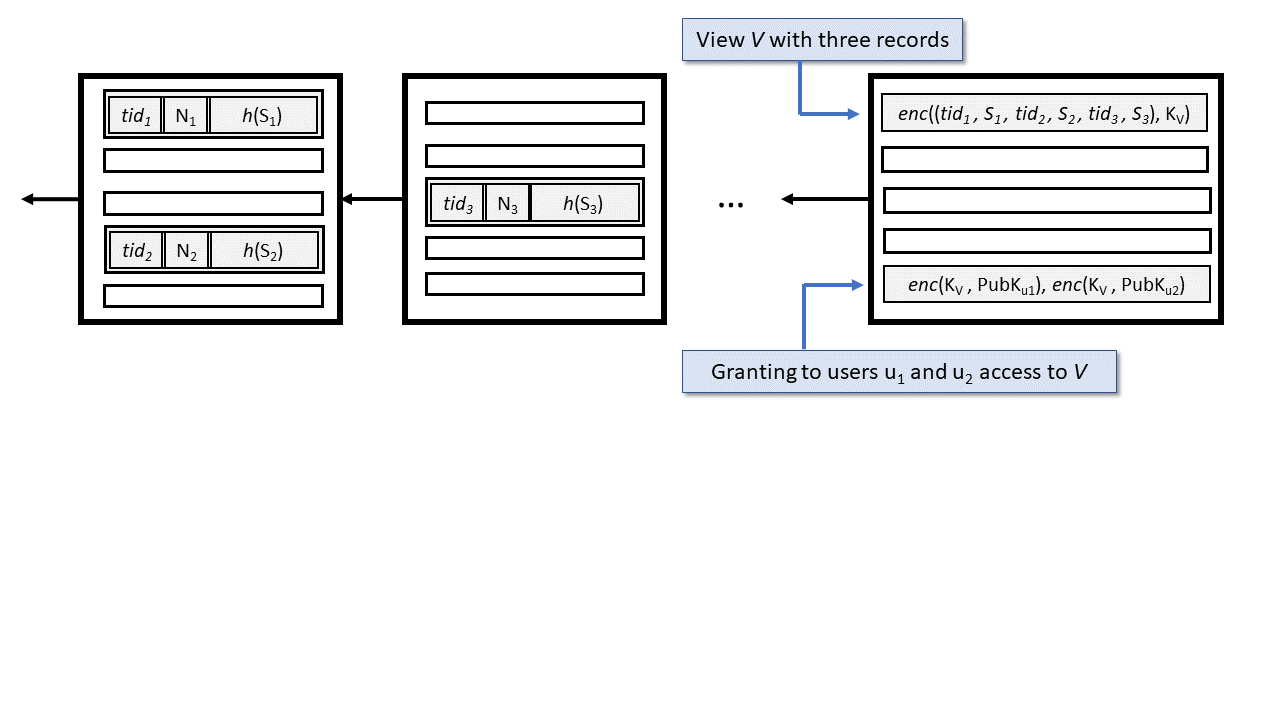
\includegraphics[trim=0 220 0 0, clip,width=0.87\textwidth]{diagram/view/hash_irrevocable.png}
    %}
    \caption{A Hash-based Irrevocable Access-control View.}
    \subcaption*{ Users who have access to the view can see the secret values and can verify that these values are correct by comparing their hash to the hash values stored on the blockchain.}
    \label{diagram:view:hash_irrevocable}
\end{figure}


\subsection{Hash-based Revocable Permissions}
\label{ch:view:ac_views:hash_revocable}

%As explained in Chapter~\ref{ch:view:ac_views:hash_irrevocable}, 
In hash-based view with revocable permissions (HR), 
the secret part of transactions is not stored on the ledger, only the hash of the concatenation of the secret with salt is revealed. The view is similar to the view in the case of ER (encryption-based revocable), as described in Chapter~\ref{ch:view:ac_views:enc_revocable}, with adaptation to hash-based storage of the secret part of transactions. Figure~\ref{diagram:view:hash_revocable} illustrates the method.

\medskip
\noindent
\textbf{Creating a view.}
Views in this method are similar to the views defined in Chapter~\ref{ch:view:ac_views:enc_revocable}. In order to make the access permission revocable, the secret information should not be disseminated to users in an irreversible way, and secret information should not be revealed by a transaction stored on the blockchain. Secret information should only be provided upon request and only to authorized users, i.e., to users with an access permission.

Consider a revocable view $V$ created by user $u$, for transactions $t_1,\ldots, t_n$. Let $u'_1,\ldots, u'_m$ be the users that should have access to the view $V$. User $u$ must know the secret part of all the transactions in $V$ to grant access to that information. But these secrets are only provided to the users $u'_1,\ldots, u'_m$ upon request, in a reversible way. 

To support revocable access permissions, the view comprises the two parts $V_{\texttt ids\/}$ and $V_{\texttt access\/}$. The list $V_{\texttt ids\/} = \{ \tid{1}, \ldots, \tid{n}\}$ is the list of ids of the transactions $t_1,\ldots, t_n$ that $V$ consists of. The list $V_{\texttt access\/}$ is created with a key $K_V$ that is selected by $u$ and disseminated to the authorized users using their public keys, $V_{\texttt access\/} = \{\enc(K_V, \pubk{u'_1}), \ldots, \enc(K_V, \pubk{u'_m})\}$. Key $K_V$ is stored in an encrypted way and only a user $u'_i$ who knows the private key $\privk{u'_i}$ can get $K_V$. 
%Note, however, that the key $K_V$ is not a key of any transaction, so knowing it still does not guarantee access to secret information.
The user $u$ who created $V$ is considered the {\em view owner\/} and any access to secret information is via $u$. 

\medskip
\noindent
\textbf{Granting and revoking access.}
When a user $u'_j$ wants to access transactions $t_{i_1}, \ldots, t_{i_k}$ of view $V$, it requests the secret values of these transactions from $u$. These values are provided encrypted as $\enc(t_{i_1}[S], K_V), \ldots, \enc(t_{i_k}[S], K_V)$. If the user 
$u'_j$ has the key $K_V$, it can decrypt the provided information and see the secret part of the requested transactions. We assume here that $K_V$ is a symmetric encryption key. Note that this does not reveal secret parts of transactions that were not included in the request. The user $u'_j$ can verify that the decrypted values  $t_{i_1}[S], \ldots, t_{i_k}[S]$ are indeed the secret values stored on the blockchain by computing $h(t_{i_j}[S]\conc s_{i_j})$ and verifying that the computed value is equal to the value stored on the blockchain for transaction $t_{i_j}$.  

To grant access to the view, $u$ can share the key $K_V$ with the new users who should gain access to $V$, where $K_V$ is encrypted using their public key.
To revoke access from users, $u$ needs to replace the key $K_V$ with a new key, say $K'_V$, and disseminate the new key $K'_V$ to the users that still have a permission to access $V$. The new key $K'_V$ is encrypted using the public keys of the authorized users, and the encrypted keys are included in $V_{\texttt access\/}$. After the change, $u$ should only use $K'_V$ to encrypt secret values it serves.   


\begin{figure}
    \centering
    %\fbox{
    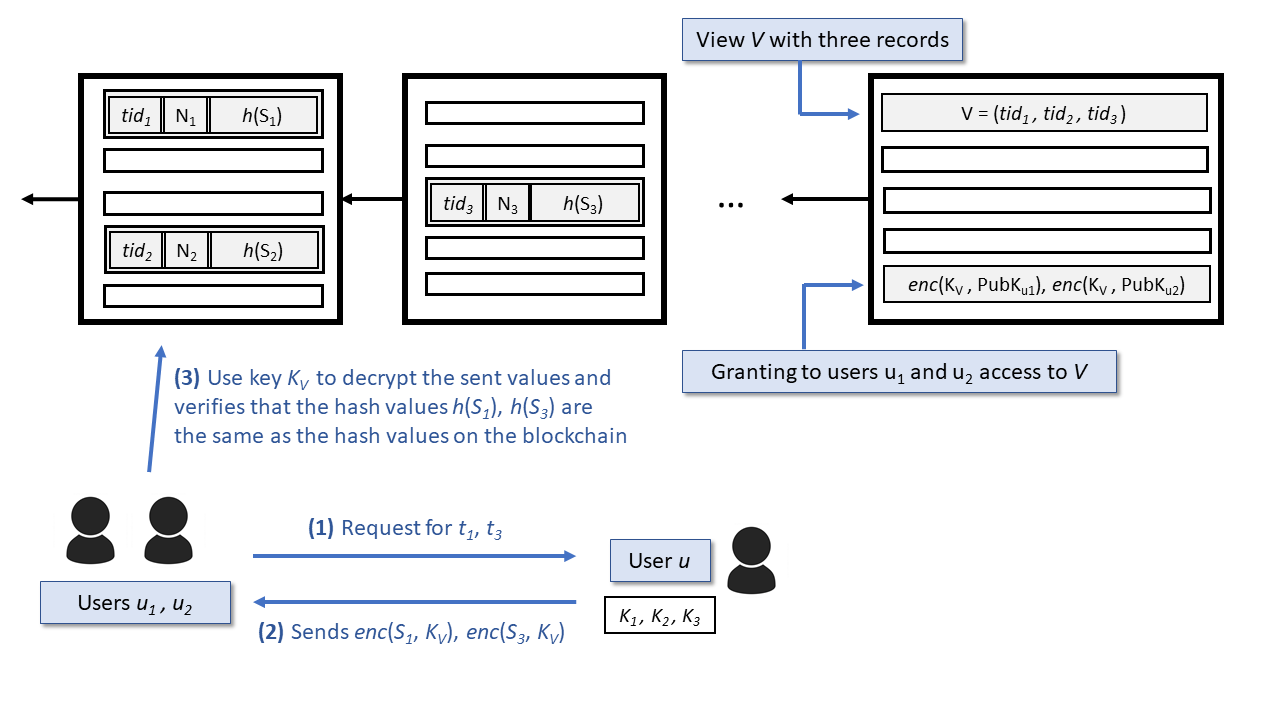
\includegraphics[trim=0 50 0 0, clip,width=0.87\textwidth]{diagram/view/hash_revocable.png}
    %}
    \caption{A Hash-based Revocable Access-control View.}
    \subcaption*{The users $u_1$ and $u_2$ request the information and it is provided encrypted by $K_V$.
    %, so only users with that key can decrypt the information. 
    They can verify that provided secret values are genuine by comparing the hash of the values to the hash of the transactions stored on the blockchain. }
    \label{diagram:view:hash_revocable}
\end{figure}


\subsection{Encryption versus Hashing}
\label{ch:view:ac_views:comparison}
In the encryption-based methods, all the information is stored on the blockchain,  where the secret data is encrypted, while in the hash-based methods, only the hash of the secret is stored on the blockchain. An advantage of encryption is that users maintain only transaction keys, while the actual data is stored on the blockchain. When storing just the hash values on the blockchain, the secret information must be stored by the users, and the hash values on the blockchain are only used for verification.
A disadvantage of encryption is the cost of creating a new key per each transaction.  

The storage space of the hash values is fixed while for the encrypted data it depends on the attribute size. Hence, if the average secret size per transaction is larger than the hash size, the encryption-based methods will use more space than the hash-based methods, and vice versa.

Both revocable and irrevocable views can be implemented using  encryption or hash-based method. The decision whether to use a revocable or an irrevocable view depends on the application. These two types of views may serve different purposes. For example, health records are typically stored in a revocable way, so that access could be revoked from healthcare workers who are no longer active, e.g., when they retire. Access to legal information, like deeds, patents and licences, should typically be irrevocable, to make the information available in the future to all the involved parties. 


\subsection{View as a Smart Contract State}
\label{ch:view:ac_views:view_as_contract}
The size of a view can be arbitrarily large. In some cases, access control views can be as large as the database itself. In such cases, it is impractical to store the entire view in a single blockchain transaction. The same may also apply to storing the list of users who have access to a particular view. To solve that, views and user lists are implemented as smart-contract states. The entire state is stored in the leaves of a Merkle tree, for each one of the local databases of the peers, and the hash at the root is stored on the ledger, as explained in Chapter~\ref{ch:view:framework}. The consensus among the peers on the view state makes it possible to verify the integrity of the views while only storing a digest on the ledger.

By representing the view as a state of the smart contract, every change in the view, like the addition of transactions to the view or the removal of transactions from the view, is represented by a new state that is propagated to all the peers. The new state is accepted as part of the consensus when the new root of the Merkle tree that reflects the change is included in the header of a block in the chain.   

\subsection{Role-Based Access Control}
\label{ch:view:ac_views:rbac}

In role-based access control (RBAC), roles are assigned to users and access permissions are given to roles~\cite{sandhu1998role,ferraiolo2003role}. A user $u$ can access an entity $e$ only if $u$ has a role with access permissions to $e$. 

Let $U$ be a set of users, $R$ be a set of roles and $D$ be a dataset. Let $\mathcal{V} \subseteq 2^D$ 
%=\{V\mid V\subseteq D\} 
be the set of views over $D$---each view is a subset of items of $D$. Assignment of roles to users is a subset $A_r \subseteq U\times R$. Access permission is a set of pairs $A_p \subseteq R\times \mathcal{V}$. A pair $(u, r)\in A_r$ means that user $u$ has role $r$, e.g., user $u$ is a nurse with access to medical records. The assignment of roles is many-to-many.
%---a user can have many roles and a role can be assigned to many users. 
An access permission $(r, V)\in A_p$ means that users with role $r$ are authorized to access view $V$. The access-permission relation is many-to-many.
%---a role can grant access to many items and an item can be accessible for many roles. 
For a role assignment $A_r$ and access permissions $A_p$, 
the set $D_u = \{V\mid \exists r . (u,r)\in A_r \wedge (r,V)\in A_p\}$
consists of the views user $u$ is allowed to access. 
%That is, a user $u$ can access item $i$ only if there is a role $r$ assigned to $u$ and role $r$ grants access to item $i$.
In a blockchain setting, access permissions relate to views that are sets of transactions.

RBAC can be implemented for all four types of access-control views presented.
%in Table~\ref{tab:four:view:types}.
To support this, first, the association $A_p$ of roles to views is stored on the blockchain as a transparent list. This list can be stored as a transaction or as a state of a smart contract. Second, the association $A_r$ between roles and public keys of users is stored on the blockchain in the same way. Any user can apply join to $A_p$ and $A_r$, to find all the public keys of users with access permissions, for any given view. These public keys are used for granting access to the views. 
Let $\mathcal{K}_{A_r\bowtie A_p}(V)$ denote the set of all public keys of users with access to $V$ according to $A_r$ and $A_p$. 

In irrevocable views, EI and HI, access to a view $V$ is granted by providing the key $K_V$ that is used for decryption of the information (keys in EI and values in HI). In the irrevocable version of RBAC, the key $K_V$ is distributed to all the users with access permissions by encrypting it with their keys and disseminating the encrypted information. Formally, this set is $\{\enc(K_v, K_i) | K_i\in \mathcal{K}_{A_r\bowtie A_p}(V)\}$. The users with access permissions have the corresponding private keys and they can decrypt $K_V$ and access the view. Other users are not privy to the key $K_V$ and cannot read the content of the encrypted view $V$.   The implementation of the key distribution for the revocable view methods ER and HR is similar. 

When a role grants access to many views, it is inefficient to distribute each key $K_V$ independently. 
Thus, a pair  $\privk{r}$ and $\pubk{r}$ of public and private keys is created for each role $r$, as if the role is a user. This can be done by any user. %, in a decentralized fashion. 
The private key $\privk{r}$ is securely shared with all the users with role $r$, e.g., by encrypting $\privk{r}$ with the public keys of these users and sending the encrypted $\privk{r}$ to them. Then, in all the four methods, the access to the view is granted to the role whose public key is $\pubk{r}$ in the same way that it is granted to a user, as described in Chapter~\ref{ch:view:ac_views}. The methods are indifferent to whether the public key belongs to a single user or to a group of users defined by a role. 

\subsection{Soundness and Completeness}
\label{ch:view:ac_views:security_model}

We analyze now the proposed approach.
A malicious user who generates or updates a view can
(1)~add to a view a transaction that should not be included in the view, (2)~add to the view a transaction that should be included in the view but in a corrupted or tampered way, or
(3)~not add to the view a transaction that should be included in the view. We explain now how verifiable soundness and completeness (defined in Chapter~\ref{ch:view:framework}) are maintained.

Case~1: Suppose that a transaction $t$ has a non-secret part $t[N]$ that does not satisfy the view definition. Including $t$ in view $V$ will violate the soundness of the view. However, because $t[N]$ is the non-secret part of the transaction, any user with access to the view can detect such transactions and verify that there are no such transactions in the view. Hence, verifiable soundness is maintained.

Case~2: If a corrupted transaction is added to the view, this could violate the soundness of the view. A case where the non-secret part of a transaction is corrupted can be detected by any user with access to the view, by comparing the non-secret part of the transaction to the non-secret part of the transaction stored on the ledger. If the secret information is corrupted, the hash of the transaction would not match the one on the ledger, in the hash-based methods. The keys would not match, in the case of corrupted keys in encryption-based methods. Hence, verifiable soundness is maintained.

Case~3: Not adding to a view all the transactions it should include will violate completeness. There are two ways to test completeness of the view at  given time $T$. First, by iterating over all the transactions in the ledger, up to time $T$, and verifying that all those that satisfy the view definition are included in the view. Second, by verifying a complete list of transactions per view maintained by a smart contract. Such a list is continuously maintained so that the completeness verification will be efficient. We elaborate on that in the next sub-chapter. By that, verifiable completeness at $T$ is maintained.   

\begin{proposition}
Given a view $V$ and a user $u$ with access permission to $V$ and to the ledger, for any time $T$, $u$ can test and verify the soundness and completeness of $V$ at $T$.
\end{proposition}

\begin{proof} (Sketch)
Let $Q$ be the query that defines the view $V$ and let $D$ be the data set of all relevant transactions. 

Completeness: User $u$ has access permission to $V$ and can execute $Q$ over the non-private part of the transactions in $D$, so $u$ can verify for every transaction $t\in Q(D)$ whose time stamp does not exceed $T$ that $t\in V$, i.e., verify $Q(D)\subseteq V$ at $T$. 

Soundness: User $u$ can test for every $t\in V$ at time $T$ that $t[N]$ satisfies the predicate of $Q$ and that $t$ is evident on the blockchain, i.e., $t\in Q(D)$. This verifies $V\subseteq Q(D)$ at $T$. 
\end{proof}


\section{Implementation}
\label{ch:view:impl}


\begin{figure}[t]
    \centering
    %\fbox{
    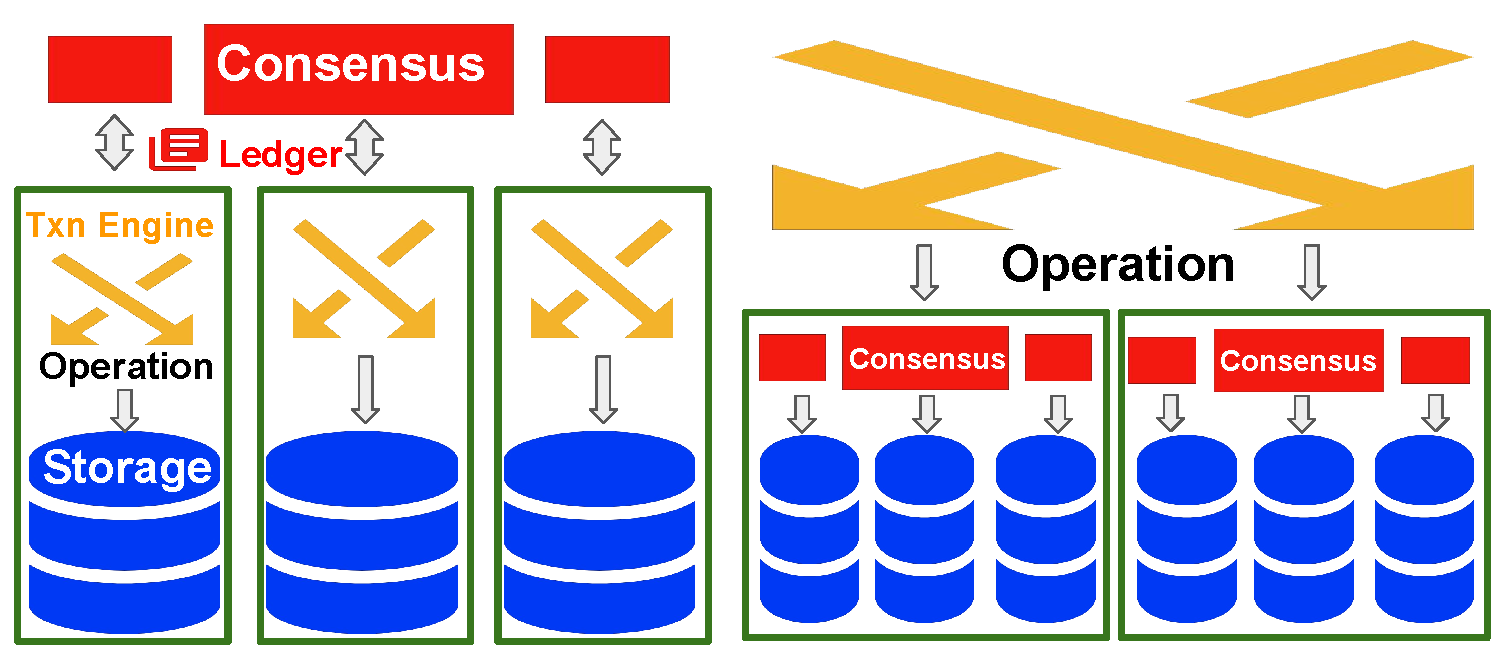
\includegraphics[width=0.87\textwidth]{diagram/view/architecture.pdf}
    %}
    \caption{System Architecture of Access-Control Views on Blockchain. }
    \subcaption*{Each blockchain node is associated with a view manager, under the same administrative domain of the view owner (dashed box). Transactions with secret data are added to the blockchain and accessed through a view manager. The view contract provides the integrity guarantee. The number of blockchain nodes may vary.}
    \label{diagram:view:impl:architecture}
\end{figure}

\begin{figure}[t]
    \centering
    %\fbox{
    \includegraphics[width=0.87\textwidth]{diagram/view/flow.pdf}
    %}
    \caption{View-management Workflow.}
    \subcaption*{For both encryption-based and hash-based view managers. Alice is a blockchain user who invokes a transaction $T$, which is included in view $V$. Bob is a view user accessing view $V$. Steps marked with an asterisk are only executed for irrevocable views, where view data are uploaded to a view contract on the chain. }
    \label{diagram:view:impl:flow}
\end{figure}
    
    
This section describes our implementation of the methods and elaborates on the system architecture. 

\subsection{System Architecture}
\label{ch:view:impl:overview}

To implement decentralized view management, a view manager component is associated with each blockchain node. Users access views via the view manager for (1)~reading from the view, and (2)~adding to the blockchain transactions with a secret part. The view manager is implemented as a set of smart contracts. An overview of the architecture is depicted in Figure~\ref{diagram:view:impl:architecture}. The interactions between components are illustrated in Figure~\ref{diagram:view:impl:flow}. Next, we elaborate on these components and interactions.




\smallskip
\noindent
\textbf{User Applications.}
There are three types of user applications.
%\begin{itemize}

\noindent
{\textbf (1)} \textit{Clients}, like Alice in Figure~\ref{diagram:view:impl:flow}, are users who invoke transactions with secret data. Client transactions have a hidden secret part. The access-control views are defined over client transactions.

\noindent
{\textbf (2)} \textit{View Owner.} View owners run a process that implements a {\texttt ViewManager} interface. 
%in Figure~\ref{fig:view_mgr}. 
The view manager intercepts and handles client requests. It translates requests into transactions, determines inclusion of transactions in views and regulates access to transactions using the methods presented in Chapter~\ref{ch:view:ac_views}. A view owner can be any user with access to all the information of the view. Hence, a view can have many view owners.

\noindent
{\textbf (3)} 
\textit{View Reader.} View readers, like Bob in Figure~\ref{diagram:view:impl:flow}, issue access requests. The requests are handed over to view owners, to be handled based on the view name and the public key of the requesting user. View readers do not always trust view owners, so provided data can be validated against the blockchain---by checking that returned secrets match the hash values on the blockchain, or that provided keys can be used for decryption of the secret data on the blockchain.  
%\end{itemize}

\smallskip
\noindent
\textbf{View Manager.} The different users interact with the {\texttt ViewManager}. 
Transactions are instantiated by contract invocations, as common in contract-based blockchains. To handle transactions with a secret part, the smart contracts of the view manager implement a common interface {\texttt WithSecret}.
The {\texttt WithSecret} interface partitions transactions into a non-secret part and a secret part, and it contains methods for processing and accessing the secret part of transactions. An {\texttt Invoke} smart contract implements the invocation logic. For a given transaction, the invocation associates the concealed secret data in the transaction with the transaction identifier in the local database of the node. 
%The format of the post-processed secret depends on the implementation of the view manager. 
Then, the contract may execute additional business logic, such as the supply-chain management procedures.
%, which is to be materialized in \textit{\_invoke} by contract developers. 

There are two main components in {\texttt ViewManager}: {\texttt CryptoHelper} which is a library of basic cryptographic primitives, and {\texttt ViewBuffer} for managing the information on each view. {\texttt ViewManager} and the interactions between the components are illustrated in Figure~\ref{diagram:view:impl:architecture}. 

The {\texttt ViewBuffer} component of {\texttt ViewManager} stores the view information. This includes (1)~{\texttt ViewKeys}, which is a map structure that associates the view name to the view key, (2)~the key $K_v$ that encrypts the list of keys in the encryption-based methods of Chapter~\ref{ch:view:ac_views:enc_irrevocable}, (3)~{\texttt ViewData}, which is a map structure that associates the view name to the relevant data.
%As later demonstrated in Figure~\ref{fig:EncryptionBasedManager} and Figure~\ref{fig:HashBasedManager}, 
The implementation of {\texttt ViewData} changes based on the view method---encryption or hashed-based.


\smallskip
\noindent
\textbf{View Management.}
View management has the following steps.

%\begin{enumerate}
\smallskip
\noindent
{\textbf (1)}  View owners create views by calling the method {\texttt CreateView} of the view manager. 
Each created view has a unique name and a logical view definition. The view definition is an implementation of the predicate that defines the view. It is a function that determines for each transaction whether it satisfies the view predicate. Transactions that satisfy the view predicate are included in the view. 
If the view owner opts for an irrevocable view, the view manager calls {\texttt Init} for instantiating the view when executing the {\texttt ViewStorage} contract (to be explained later), which manages the view storage. 

\smallskip
\noindent
{\textbf (2)} Transactions with a secret part are inserted into the blockchain through {\texttt InvokeWithSecret}. The view manager processes the secret data provided by the client, based on its subclass implementation of {\texttt ProcessSecret}, to cope with different view types. The processed secret and the other arguments adhere to the {\texttt WithSecret} interface. The view owner retrieves the transaction identifier based on the formatted parameters, and determines all the view-definition predicates that are satisfied by the parameters. For each view whose predicate is satisfied, the view manager calls {\texttt InsertIntoView}, to include the transaction identifier in the view. For example, clients, like Alice in Figure~\ref{diagram:view:impl:flow}, contact the view owner and invoke a transaction, e.g., for insertion into the blockchain or for adding to a view. The request is processed by the view owner who invokes {\texttt InvokeWithSecret} in its {\texttt ViewManager} process. The view manager of a view owner processes the request and securely delivers the data to a {\texttt ViewStorage} contract that handles the data storage.

\smallskip
\noindent
{\textbf (3)} A view user, like Bob in Figure~\ref{diagram:view:impl:flow}, may pose a  query to a view by invoking {\texttt QueryView} via the view manager. Despite implementation differences, the public key of the user is provided with the query for authentication. Query results are encrypted with that key. 
%\end{enumerate}

%The above steps present the general architecture and procedure of our view management approach. However, there are plenty of missing details, such as how view managers process the client-provided secret data, append a transaction into a view, respond a view query from a user, and how view users validate the queried results. The above procedures differ between the subclasses of {\texttt ViewManager}, either {\texttt EncryptionBasedManager} or {\texttt HashBasedManager}.  It especially concerns on their implementations of {\tt\_process}, {\tt\_insertIntoView} and {\texttt QueryView} in Figure~\ref{fig:view_mgr}, which are clarified in next subsections. 

\smallskip
\noindent
\textbf{View Storage Contract.} A view-storage contract is called for storing data of irrevocable views. The type of view (revocable versus irrevocable) is set when {\texttt CreateView} is first called.  
The {\texttt ViewStorage} contract maintains a map structure {\texttt ViewInfo} that associates the view name with the view data. 
The view data is also a map structure whose internal structure for the key-value pairs depends on the implementation of {\texttt ViewManager}, to support the different view types. 
 {\texttt ViewStorage} supports two methods. An {\texttt Init} method initializes for a given view name an empty view data, i.e., an empty map. A {\texttt Merge} method adds data to the view by incorporating in {\texttt ViewInfo} missing key-value pairs from {\texttt ViewData}. 
%In a {\texttt Merge}, operation in Figure~\ref{fig:view_contract}, the steps adds the non-existed  key-value pairs of {\texttt ViewData} are included in {\texttt ViewInfo}.
By maintaining the irrevocable view data in a contract, we use security features of the blockchain to protect the view integrity. Thus, query results that are returned to view users are protected from tampering. 


\subsubsection{Encryption-based View Manager}

The implementation of the view manger depends on the view type.
We elaborate now on encryption-based view manager.

\medskip
\noindent
\textbf{Overview} 
{\texttt EncryptionBasedManager} is a class that implements the {\texttt ViewManager} interface and the methods of Chapter~\ref{ch:view:ac_views:enc_irrevocable} and~\ref{ch:view:ac_views:enc_revocable}. 
The format of the view and the {\texttt ViewBuffer} are designed to support the encryption-based methods. 
The view data is a mapping from the transaction identifier ${\texttt tid\/}_i$ to the transaction key $K_i$, in the notation of Chapter~\ref{ch:view:ac_views:enc_irrevocable}. The procedures  {\texttt InsertIntoView}, {\texttt ProcessSecret}, and {\texttt QueryView} are adapted to this format.

\medskip
\noindent
\textbf{Secret Processing.}
In {\texttt ProcessSecret}, a new symmetric key is created for each new transaction.
%in Figure~\ref{EncryptionBasedManager} that we create a symmetric key for each transaction. 
The procedure encrypts the secret part of the transaction and returns the encrypted text and key. 

\medskip
\noindent
\textbf{View Update.}
When {\texttt InsertIntoView} is executed, 
the transaction identifier and the generated transaction key are stored in the {\texttt ViewBuffer}.
%, for views with either revocable or irrevocable access permissions. 
In the irrevocable case, 
the view key (which is generated if needed) is used for encrypting the identifier and the key of the transaction. 
The encrypted result is provided to the {\texttt Merge} procedure of the {\texttt ViewStorage} contract.
For views with irrevocable access permissions, the view data are automatically updated on the chain to obtain the blockchain-provided immutability. 

\medskip
\noindent
\textbf{Querying a View.}
There are differences between revocable and irrevocable view management, when answering user queries. 
For revocable access permissions, a symmetric key is generated per each query.
This key is used for encrypting the view data, which is a mapping from transaction identifiers to transaction keys.
For irrevocable access permissions, the view key has already been created in {\texttt InsertIntoView}, so it is directly retrieved from {\texttt ViewBuffer}. 
In both cases, the user-provided public key is applied, in order to encrypt the returned data and protect the view keys. 

\medskip
\noindent
\textbf{Validation.}
Users validate query results against the content of the blockchain, to verify that the results were not tampered with. After receiving a reply from a view owner, when calling {\texttt QueryView}, the user validates the secret data, for each transaction in the view. 
First, view keys are revealed by decryption, using the private key of the user. 
The query answer contains the encrypted view data, hence,
the user can decrypt the view data with the provided view keys.
For views with irrevocable permissions, users retrieve the encrypted view data from the {\texttt ViewStorage} contract, and then execute decryption. 
With the decrypted identifiers and keys, of the requested transactions, the user can pull from any blockchain node the relevant transactions and decrypt their secret part. 


\subsubsection{Hash-based View Manager}

The hash-based view manager  {\texttt HashBasedManager} has the same architecture as the encryption-based manager.
%, where {\texttt EncryptionBasedManager} is replaced by {\texttt HashBasedManager}.
The storage, the buffer and methods like view update, querying and validation are modified accordingly.



\subsection{Transaction List per View}
\label{ch:view:impl:view_merge}
To test completeness for views, it is efficient to maintain for each view its list of transactions. But transactions cannot be added to views through smart contracts because that would require revealing the view key to the blockchain peers, which would expose information to unauthorized users. Thus, insertion of transactions to the main database is through a smart contract that updates lists of transaction ids per view, but does not update the views themselves, e.g., if transaction $t_i$ is added to the blockchain and should be included in views $V_1$ and $V_2$, then $\tid{i}$ will be added to the transaction lists of $V_1$ and $V_2$, based on the non-secret part $t_i[N]$.
We refer to this smart contract as 
\texttt{ViewInContract}.

The smart contract maintains a list of views, their predicates and their list of transaction ids. For each added transaction, its id is added to all the lists for which the view predicate is satisfied. To cope with the low update rate of blockchains, the list updates are conducted in batches. Initially, updates are collected and transaction ids are associated with the insertion time stamp. Every time interval, say 30 seconds, all the accumulated updates are written to the ledger. Completeness can be tested for the time of the latest update.


\subsection{Hyperledger Fabric}
\label{ch:view:impl:fabric}

We implemented the system using Hyperledger Fabric v2.2---a permissioned blockchain system~\cite{androulaki2018hyperledger}, which is customized for enterprise-grade applications. 
Although we used Fabric with its unique design choices for our proof of concept, our implementation is generic, because we do not rely on any feature that is unique to Fabric and does not exist in other blockchain systems. 
In particular, our system uses smart contracts in a general way, 
without relying on the chaincode lifecycle. 
We only rely on tamper-evidence guarantees of smart contracts for the integrity of view data, but these are provided by any blockchain that supports smart contracts. Any mechanism to guarantee state integrity, such as Merkle tree, can be used for securing the integrity of blockchain views.


\section{Experimental Evaluation}
\label{ch:view:experiments}

\smallskip
\noindent
\textbf{Goals.}
The goals of the experiments are as follows. 
(1)~Study the effect of our methods on the performance of blockchains, in terms of transaction rate, latency and storage space.  
(2)~Compare the proposed access-control views with a baseline in which different views are stored on independent ledgers and cross-blockchain transactions are executed for keeping the consistency of the views and the main ledger.
(3)~Explore the overhead of managing a list of transaction ids per view, as described in Chapter~\ref{ch:view:impl:view_merge}. 

\subsection{Baseline}
As a baseline, we consider the case where each view is stored on a separate blockchain, called \textit{view blockchain}, and each blockchain is accessible only to users with access permissions for the corresponding view. 
To keep the views consistent with the main blockchain, which stores all the transactions, we use cross-chain transactions. If a transaction $t$ is included in $n$ different views, a cross-blockchain insertion transaction will guarantee consistency among all the view blockchains---$t$ should either be included in all the $n$ corresponding blockchains or in none of them. Hence, the operation is atomic. 

We implemented the cross-blockchain transactions protocol of AHL~\cite{dang2019towards} where each cross-blockchain transaction follows the two-phase commit (2PC) protocol.
The main blockchain operates like a database transaction coordinator of 2PC.
For each database update, it employs a smart contract to determine the updated views and the view blockchains that store them. It then issues to all of them a  {\texttt Prepare} request. 
Each view blockchain operates as a 2PC shard where the 2PC protocol logic is implemented as a smart contract. % called {\texttt TxnCoordinator}. 
After gathering sufficient positive responses from the view blockchains, the main blockchain issues a {\texttt Commit} request to all the view blockchains, and the update is included in their ledger. 

If a cross-blockchain transaction involves $n$ blockchains, it is translated into $2n$ blockchain transactions, following the 2PC protocol. The first $n$ transactions simulate the {\texttt Prepare} requests on each one of $n$ blockchains. The following $n$ transactions simulate the corresponding {\texttt Commit} requests of the 2PC protocol. 
Note that $n$ {\texttt Prepare} requests or $n$ {\texttt Commit} requests can occur concurrently. 

If the majority of the peers in all the blockchains are following the protocol, the 2PC procedure provides verifiable soundness and completeness. Each view blockchain will include only transactions of the view and will include all the transactions (otherwise, the commit phase of 2PC will not be carried out).
Without 2PC, where view blockchains are independent from the main chain, neither soundness nor completeness will be guaranteed. We cannot rely on having a trusted entity to assure that all the view blockchains are consistent with the main blockchain, hence, 2PC is required. 


\begin{figure*}[tp]
	\begin{minipage}[t]{0.32\textwidth}
		\centering
        \includegraphics[width=0.99\textwidth]{chart/view/thruput.pdf}
		\caption{Throughput.}
		\label{chart:view:exp:thruput} 
	\end{minipage}
    \hfill
	\begin{minipage}[t]{0.32\textwidth}
		\centering
        \includegraphics[width=0.99\textwidth]{chart/view/latency.pdf}
		\caption{Latency.}
        \label{chart:view:exp:latency}
	\end{minipage}
	\hfill
	\begin{minipage}[t]{0.32\textwidth}
		\centering
    \includegraphics[width=0.99\textwidth]{chart/view/storage.pdf}
    \caption{Storage Overhead.}
    \label{chart:view:exp:storage}
	\end{minipage}
\end{figure*}



\subsection{Supply Chain Workload}
We benchmarked the access-control views on a variety of supply chain workloads. 
%, similar to the supply chain illustrated in Figure~\ref{fig:supply:chain}.
To that end, we implemented a workload generator that produces workloads of supply chain transactions according to given parameters. When a workload is created, first the topology of the supply-chain graph is defined. The user specifies the nodes and the edges of the graph of the supply chain. Each node represents a real-world entity that is part of the supply chain and has a need to access information. Each edge from node $n_i$ to node $n_j$ represents a delivery link from node $n_i$ to node $n_j$, for delivering received items from $n_i$ to $n_j$. An item cannot be forwarded by node $n_i$ to more than one following node. 

Some nodes are dispatching nodes, e.g., manufacturers. These nodes can create items and send them on to following nodes in the chain. All the other nodes can only forward items that they received. Some nodes are terminal nodes. They receive items and do not transfer them on to a following node, e.g., shops in Figure~\ref{diagram:view:supply_chain:}. The user can select how many items will be dispatched and the behavior of intermediate nodes. Each transfer is recorded on the blockchain.
In the creation of the workload, when an item is forwarded, all the nodes that handled it can see the transfer transaction. That is, nodes can continue tracking an item they delivered. Nodes can also see all the historical transfers of the items they received. However, a node should not have access to any other delivery transactions. 

The generated records of the supply-chain transactions are stored on a blockchain and access restrictions are implemented using the access-control view methods. For each node $n$ there is a view $V_n$ that contains all the transactions that node $n$ has access to. When a transfer of an item occurs, the transaction is added to the main chain and all the relevant views are updated. For example, suppose that item $i$ was created in node $n_0$, then it was transferred to node $n_1$, then to node $n_2$, and the most recent transaction is a transfer of $i$ from node $n_2$ to node $n_3$. Then, the transaction $(i, n_2, n_3)$ is added to the blockchain. The access to it is granted to nodes $n_0$, $n_1$, $n_2$ and $n_3$. So, the access-control views of all these nodes, i.e., $V_{n_0}$, $V_{n_1}$, $V_{n_2}$ and $V_{n_3}$, are updated by adding this transaction to them. In addition, the view of node $n_3$ is updated by adding the historical transfers of item $i$ to it, that is, granting access to $n_3$ for these transactions. This means that the transactions $(i, n_0, n_1)$ and $(i, n_1, n_2)$ are added to view $V_{n_3}$, to reflect the added access permissions of $n_3$ for item $i$.  

The workload generator was used for benchmarking the access control views on supply chains with varying topology, size and volume of transactions. Note that the size of the supply chain, i.e., the number of nodes in it, determines the number of views.


\medskip
\noindent
\textbf{Transaction Rate.}
We measured the transaction rate---the number of committed application requests per second (TPS)---as a function of the number of clients. 
%We examined the ability of the blockchain to cope with different transaction rates, with and without access-control views.
We increased the number of client processes to handle the supply-chain workload. 
Each client groups 25 requests into a batch and transaction batches are invoked in a sequential manner. 
Figure~\ref{chart:view:exp:thruput} presents the result throughput as a function of the number of client processes. 
All our view methods achieve higher scalability than the baseline.  The view methods with revocable access gained the highest throughput, reaching nearly 500 requests per second. 
For views with irrevocable access, the system achieved around 150 requests per second. 
The lower throughput of irrevocable views is because in addition to the procedures performed by the revocable methods, they call view-modifying transactions, which require extra computations.
The  \texttt{ViewInContract} presented in Chapter~\ref{ch:view:impl:view_merge}
for managing the list of transactions per view, for testing completeness efficiently, has a very low overhead.

The baseline (cross-chain based) approach requires many more transactions per request, i.e., a request is translated into $2n$ transactions, for updating $n$ views. Hence, the baseline does not scale well, and it has a much lower throughput of less than 50 requests per second even with 32 concurrent clients. 


\begin{figure*}[tp]
	\begin{minipage}[t]{0.32\textwidth}
		\centering
        \includegraphics[width=0.99\textwidth]{chart/view/txn_relationship.pdf}
        % \caption{Throughput in terms of Supply Chain Transaction}
        \caption{Transactions per Request.}
        \label{chart:view:exp:txn_relationship}
	\end{minipage}
	\hfill
	\begin{minipage}[t]{0.32\textwidth}
		\centering
        \includegraphics[width=0.95\textwidth]{chart/view/scale_single_view.pdf}
        \caption{Each Transaction in a Single View.}
        \label{chart:view:exp:single_view}
	\end{minipage}
    \hfill
	\begin{minipage}[t]{0.32\textwidth}
		\centering
        \includegraphics[width=0.99\textwidth]{chart/view/scale_full_view.pdf}
        \caption{Each Transaction in All the Views.}
        \label{chart:view:exp:all_view}
	\end{minipage}
\end{figure*}


\medskip
\noindent
\textbf{Latency.}
% The latency is the time it takes for a new transaction to be included in the blockchain. We tested the effect of the access-control views on the latency. 
Figure~\ref{chart:view:exp:latency} depicts the per-request latency for the four view methods and the baseline, per the number of clients. 
The irrevocable views have a higher latency than the revocable views. This is due to the extra view-modifying on-chain transactions, which add about 1 second to the latency. The running time of off-chain computations, such as encryption and hash computations, is below 50ms.
This is negligible compared to on-chain transaction delay, which is around 1 second. 
Since \texttt{ViewInContract} moves  view management logic from view owners to user contracts, it saves the extra view-modifying on-chain transactions. Furthermore, despite its complex contract logic, \texttt{ViewInContract} has latency close to that of revocable views. It is because the blockchain transactions are more susceptible to factors other than data processing, such as consensus and cryptographic operations, especially in Hyperledger Fabric~\cite{sharma2019blurring}. 
The baseline approach has higher latency than our methods, and its latency soars as the number of clients increases. This is because the high load on the blockchains that occurs when increasing the number of clients overwhelms the system. 



\medskip
\noindent
\textbf{Storage Overhead.}
We examined the total blockchain storage that was used, as we increase the number of views. 
We measured the storage consumption for a growing number of views, after committing 40 supply-chain requests. 
This number is equal to the number of ledgers in the cross-chain baseline after loading 400 supply chain requests by each one of four client processes. 
Figure~\ref{chart:view:exp:storage} presents the results. 
As expected, without the view-storage contract, the revocable methods need the least space and are not affected by the number of views. 
The used space for the irrevocable view methods grows as the number of views increases.
The same occurs when employing \texttt{ViewInContract}. For managing the list of transaction ids per view, we store view data and view predicates, so having more views requires more storage to be used by \texttt{ViewInContract}, more than what is needed by the other methods.
Nonetheless, the baseline approach is the most wasteful in storage space because it needs to duplicate transactions---a transaction in $n$ views is duplicated $n$ times. Therefore, the total space needed for the baseline approach is tenfold greater than the storage space used by our view methods. 


\medskip
\noindent
\textbf{Processing Cost.}
Communication between the blockchain nodes and the load on nodes are affected by the total number of on-chain transactions. In this experiment, we measured the number of on-chain transaction as a function of the number of Application Requests.  
The results are provided in Figure~\ref{chart:view:exp:txn_relationship}.
In the workload, a request involves 10 views, on the average. 
Without the extra view-modifying contract, in revocable views and \texttt{ViewInContract}, the number of application requests is equal to the number of on-chain transactions. In irrevocable views, we need an extra on-chain transaction to invoke the view storage contract, so the number of on-chain transactions is doubled---$r$ requests will result in $2r$ on-chain transactions.  
%This is to instruct the inclusion of the request into the specified views. 
The cross-chain baseline, for comparison, requires $2\cdot |V|\cdot n$, where $|V|$ is the average number of views per transaction,  and $n$ is the number of requests. In Figure~\ref{chart:view:exp:txn_relationship}, $|V|=10$. 



\medskip
\noindent
\textbf{Scalability.}
We examined the effect of an increase in the number of views on the performance. 
This is related to \texttt{ViewInContract} due to the testing of the view predicates for each transaction invocation. Thus, we examined the effect of \texttt{ViewInContract} by increasing the number of views from 1 to 100. 
We measured latency and throughput for the two cases presented in Figure~\ref{chart:view:exp:single_view} and Figure~\ref{chart:view:exp:all_view}.

In Figure~\ref{chart:view:exp:single_view} each transaction belongs to a single view. An increase in the number of views did not affect the performance: latency of about 900 ms and throughput of about 420 TPS in all scenarios. 
% The only increase was in the amount of work each peer had to execute. 
In Figure~\ref{chart:view:exp:all_view}, each transaction is included in all the views. An increase in the number of views from 1 to 100 changes the latency from around 900 ms to about 2800 ms and the throughput from approximately 450 TPS to 130 TPS.
The results are similar for both the hash-based and encryption-based methods.

The reason for the difference between the scenario in Figure~\ref{chart:view:exp:single_view} and that of Figure~\ref{chart:view:exp:all_view} is that when updating many views per transaction, the transaction needs to include more information in its payload. This increases the size of transactions and reduces the number of transactions per block, affecting the throughput and the latency.